\chapter{Conectividade forte}

\index{grafo fortemente conexo}

Em um grafo direcionado,
as arestas podem ser percorridas em apenas uma direção,
então mesmo se o grafo for conexo,
isso não garante que haverá
um caminho de um nó para outro nó.
Por essa razão, é significativo definir um novo conceito
que requer mais do que conectividade.

Um grafo é \key{fortemente conexo}
se houver um caminho de qualquer nó para todos
os outros nós no grafo.
Por exemplo, na figura a seguir,
o grafo à esquerda é fortemente conexo,
enquanto o grafo à direita não é.

\begin{center}
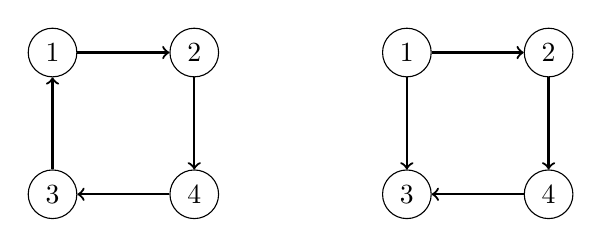
\begin{tikzpicture}[scale=0.9]
\node[draw, circle] (1) at (1,1) {$1$};
\node[draw, circle] (2) at (3,1) {$2$};
\node[draw, circle] (3) at (1,-1) {$3$};
\node[draw, circle] (4) at (3,-1) {$4$};

\path[draw,thick,->] (1) -- (2);
\path[draw,thick,->] (2) -- (4);
\path[draw,thick,->] (4) -- (3);
\path[draw,thick,->] (3) -- (1);

\node[draw, circle] (1b) at (6,1) {$1$};
\node[draw, circle] (2b) at (8,1) {$2$};
\node[draw, circle] (3b) at (6,-1) {$3$};
\node[draw, circle] (4b) at (8,-1) {$4$};

\path[draw,thick,->] (1b) -- (2b);
\path[draw,thick,->] (2b) -- (4b);
\path[draw,thick,->] (4b) -- (3b);
\path[draw,thick,->] (1b) -- (3b);
\end{tikzpicture}
\end{center}

O grafo à direita não é fortemente conexo
porque, por exemplo, não há caminho
do nó 2 para o nó 1.

\index{componente fortemente conexo}
\index{grafo de componentes}

Os \key{componentes fortemente conexos}
de um grafo dividem o grafo em partes fortemente conexas
que são tão grandes quanto possível.
Os componentes fortemente conexos formam um
\key{grafo de componentes} acíclico que representa
a estrutura profunda do grafo original.

Por exemplo, para o grafo
\begin{center}
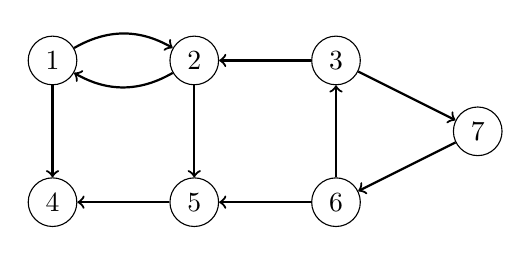
\begin{tikzpicture}[scale=0.9,label distance=-2mm]
\node[draw, circle] (1) at (-1,1) {$7$};
\node[draw, circle] (2) at (-3,2) {$3$};
\node[draw, circle] (4) at (-5,2) {$2$};
\node[draw, circle] (6) at (-7,2) {$1$};
\node[draw, circle] (3) at (-3,0) {$6$};
\node[draw, circle] (5) at (-5,0) {$5$};
\node[draw, circle] (7) at (-7,0) {$4$};

\path[draw,thick,->] (2) -- (1);
\path[draw,thick,->] (1) -- (3);
\path[draw,thick,->] (3) -- (2);
\path[draw,thick,->] (2) -- (4);
\path[draw,thick,->] (3) -- (5);
\path[draw,thick,->] (4) edge [bend left] (6);
\path[draw,thick,->] (6) edge [bend left] (4);
\path[draw,thick,->] (4) -- (5);
\path[draw,thick,->] (5) -- (7);
\path[draw,thick,->] (6) -- (7);
\end{tikzpicture}
\end{center}
os componentes fortemente conexos são os seguintes:
\begin{center}
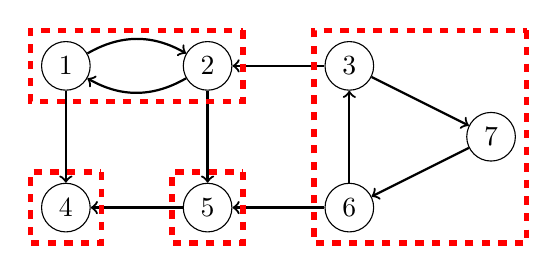
\begin{tikzpicture}[scale=0.9]
\node[draw, circle] (1) at (-1,1) {$7$};
\node[draw, circle] (2) at (-3,2) {$3$};
\node[draw, circle] (4) at (-5,2) {$2$};
\node[draw, circle] (6) at (-7,2) {$1$};
\node[draw, circle] (3) at (-3,0) {$6$};
\node[draw, circle] (5) at (-5,0) {$5$};
\node[draw, circle] (7) at (-7,0) {$4$};

\path[draw,thick,->] (2) -- (1);
\path[draw,thick,->] (1) -- (3);
\path[draw,thick,->] (3) -- (2);
\path[draw,thick,->] (2) -- (4);
\path[draw,thick,->] (3) -- (5);
\path[draw,thick,->] (4) edge [bend left] (6);
\path[draw,thick,->] (6) edge [bend left] (4);
\path[draw,thick,->] (4) -- (5);
\path[draw,thick,->] (5) -- (7);
\path[draw,thick,->] (6) -- (7);

\draw [red,thick,dashed,line width=2pt] (-0.5,2.5) rectangle (-3.5,-0.5);
\draw [red,thick,dashed,line width=2pt] (-4.5,2.5) rectangle (-7.5,1.5);
\draw [red,thick,dashed,line width=2pt] (-4.5,0.5) rectangle (-5.5,-0.5);
\draw [red,thick,dashed,line width=2pt] (-6.5,0.5) rectangle (-7.5,-0.5);
\end{tikzpicture}
\end{center}
O grafo de componentes correspondente é o seguinte:
\begin{center}
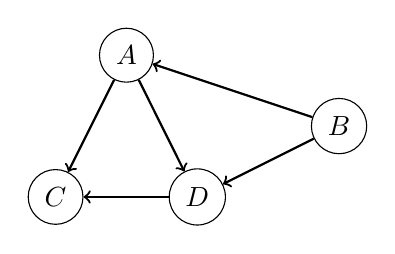
\begin{tikzpicture}[scale=0.9]
\node[draw, circle] (1) at (-3,1) {$B$};
\node[draw, circle] (2) at (-6,2) {$A$};
\node[draw, circle] (3) at (-5,0) {$D$};
\node[draw, circle] (4) at (-7,0) {$C$};

\path[draw,thick,->] (1) -- (2);
\path[draw,thick,->] (1) -- (3);
\path[draw,thick,->] (2) -- (3);
\path[draw,thick,->] (2) -- (4);
\path[draw,thick,->] (3) -- (4);
\end{tikzpicture}
\end{center}
Os componentes são $A=\{1,2\}$,
$B=\{3,6,7\}$, $C=\{4\}$ e $D=\{5\}$.

Um grafo de componentes é um grafo direcionado acíclico,
então é mais fácil de processar do que o grafo original.
Como o grafo não contém ciclos,
sempre podemos construir uma ordenação topológica e
usar técnicas de programação dinâmica como aquelas
apresentadas no Capítulo 16.

\section{Algoritmo de Kosaraju}

\index{algoritmo de Kosaraju}

O \key{algoritmo de Kosaraju}\footnote{De acordo com \cite{aho83},
S. R. Kosaraju inventou este algoritmo em 1978,
mas não o publicou. Em 1981, o mesmo algoritmo foi redescoberto
e publicado por M. Sharir \cite{sha81}.} é um método eficiente
para encontrar os componentes fortemente conexos
de um grafo direcionado.
O algoritmo realiza duas buscas em profundidade:
a primeira busca constrói uma lista de nós
de acordo com a estrutura do grafo,
e a segunda busca forma os componentes fortemente conexos.

\subsubsection{Busca 1}

A primeira fase do algoritmo de Kosaraju constrói
uma lista de nós na ordem em que uma
busca em profundidade os processa.
O algoritmo percorre os nós,
e inicia uma busca em profundidade em cada 
nó não processado.
Cada nó será adicionado à lista
após ter sido processado.

No grafo de exemplo, os nós são processados
na seguinte ordem:
\begin{center}
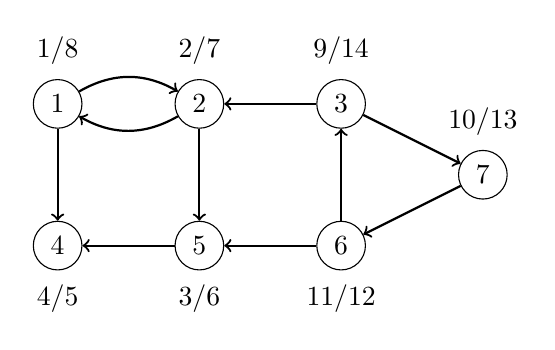
\begin{tikzpicture}[scale=0.9,label distance=-2mm]
\node[draw, circle] (1) at (-1,1) {$7$};
\node[draw, circle] (2) at (-3,2) {$3$};
\node[draw, circle] (4) at (-5,2) {$2$};
\node[draw, circle] (6) at (-7,2) {$1$};
\node[draw, circle] (3) at (-3,0) {$6$};
\node[draw, circle] (5) at (-5,0) {$5$};
\node[draw, circle] (7) at (-7,0) {$4$};

\node at (-7,2.75) {$1/8$};
\node at (-5,2.75) {$2/7$};
\node at (-3,2.75) {$9/14$};
\node at (-7,-0.75) {$4/5$};
\node at (-5,-0.75) {$3/6$};
\node at (-3,-0.75) {$11/12$};
\node at (-1,1.75) {$10/13$};

\path[draw,thick,->] (2) -- (1);
\path[draw,thick,->] (1) -- (3);
\path[draw,thick,->] (3) -- (2);
\path[draw,thick,->] (2) -- (4);
\path[draw,thick,->] (3) -- (5);
\path[draw,thick,->] (4) edge [bend left] (6);
\path[draw,thick,->] (6) edge [bend left] (4);
\path[draw,thick,->] (4) -- (5);
\path[draw,thick,->] (5) -- (7);
\path[draw,thick,->] (6) -- (7);
\end{tikzpicture}
\end{center}

A notação $x/y$ significa que
o processamento do nó começou
no tempo $x$ e terminou no tempo $y$.
Assim, a lista correspondente é a seguinte:

\begin{tabular}{ll}
\\
nó & tempo de processamento \\
\hline
4 & 5 \\
5 & 6 \\
2 & 7 \\
1 & 8 \\
6 & 12 \\
7 & 13 \\
3 & 14 \\
\\
\end{tabular}
% 
% Na segunda fase do algoritmo,
% os nós serão processados
% em ordem inversa: $[3,7,6,1,2,5,4]$.

\subsubsection{Busca 2}

A segunda fase do algoritmo
forma os componentes fortemente conexos
do grafo.
Primeiro, o algoritmo inverte cada
aresta no grafo.
Isso garante que durante a segunda busca,
sempre encontraremos componentes fortemente conexos
que não possuem nós extras.

Após inverter as arestas,
o grafo de exemplo é o seguinte:
\begin{center}
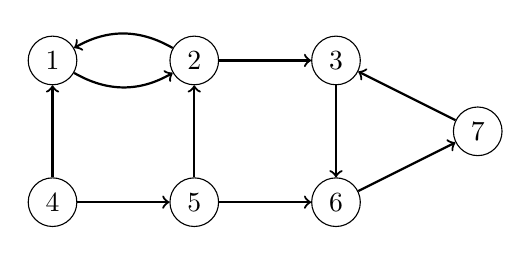
\begin{tikzpicture}[scale=0.9,label distance=-2mm]
\node[draw, circle] (1) at (-1,1) {$7$};
\node[draw, circle] (2) at (-3,2) {$3$};
\node[draw, circle] (4) at (-5,2) {$2$};
\node[draw, circle] (6) at (-7,2) {$1$};
\node[draw, circle] (3) at (-3,0) {$6$};
\node[draw, circle] (5) at (-5,0) {$5$};
\node[draw, circle] (7) at (-7,0) {$4$};

\path[draw,thick,<-] (2) -- (1);
\path[draw,thick,<-] (1) -- (3);
\path[draw,thick,<-] (3) -- (2);
\path[draw,thick,<-] (2) -- (4);
\path[draw,thick,<-] (3) -- (5);
\path[draw,thick,<-] (4) edge [bend left] (6);
\path[draw,thick,<-] (6) edge [bend left] (4);
\path[draw,thick,<-] (4) -- (5);
\path[draw,thick,<-] (5) -- (7);
\path[draw,thick,<-] (6) -- (7);
\end{tikzpicture}
\end{center}

Depois disso, o algoritmo percorre
a lista de nós criada pela primeira busca,
em ordem \emph{inversa}.
Se um nó não pertence a um componente,
o algoritmo cria um novo componente
e inicia uma busca em profundidade
que adiciona todos os novos nós encontrados durante a busca
ao novo componente.

No grafo de exemplo, o primeiro componente
começa no nó 3:

\begin{center}
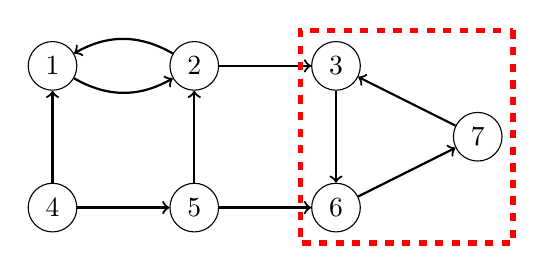
\begin{tikzpicture}[scale=0.9,label distance=-2mm]
\node[draw, circle] (1) at (-1,1) {$7$};
\node[draw, circle] (2) at (-3,2) {$3$};
\node[draw, circle] (4) at (-5,2) {$2$};
\node[draw, circle] (6) at (-7,2) {$1$};
\node[draw, circle] (3) at (-3,0) {$6$};
\node[draw, circle] (5) at (-5,0) {$5$};
\node[draw, circle] (7) at (-7,0) {$4$};

\path[draw,thick,<-] (2) -- (1);
\path[draw,thick,<-] (1) -- (3);
\path[draw,thick,<-] (3) -- (2);
\path[draw,thick,<-] (2) -- (4);
\path[draw,thick,<-] (3) -- (5);
\path[draw,thick,<-] (4) edge [bend left] (6);
\path[draw,thick,<-] (6) edge [bend left] (4);
\path[draw,thick,<-] (4) -- (5);
\path[draw,thick,<-] (5) -- (7);
\path[draw,thick,<-] (6) -- (7);

\draw [red,thick,dashed,line width=2pt] (-0.5,2.5) rectangle (-3.5,-0.5);
\end{tikzpicture}
\end{center}

Observe que como todas as arestas são invertidas,
o componente não ''vaza'' para outras partes no grafo.

\begin{samepage}
Os próximos nós na lista são os nós 7 e 6,
mas eles já pertencem a um componente,
então o próximo novo componente começa no nó 1:

\begin{center}
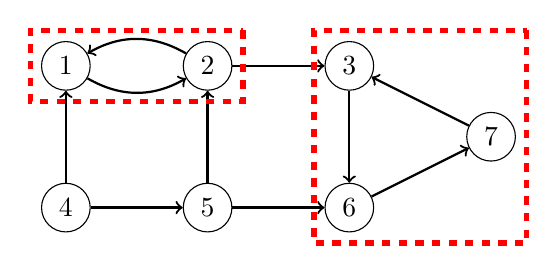
\begin{tikzpicture}[scale=0.9,label distance=-2mm]
\node[draw, circle] (1) at (-1,1) {$7$};
\node[draw, circle] (2) at (-3,2) {$3$};
\node[draw, circle] (4) at (-5,2) {$2$};
\node[draw, circle] (6) at (-7,2) {$1$};
\node[draw, circle] (3) at (-3,0) {$6$};
\node[draw, circle] (5) at (-5,0) {$5$};
\node[draw, circle] (7) at (-7,0) {$4$};

\path[draw,thick,<-] (2) -- (1);
\path[draw,thick,<-] (1) -- (3);
\path[draw,thick,<-] (3) -- (2);
\path[draw,thick,<-] (2) -- (4);
\path[draw,thick,<-] (3) -- (5);
\path[draw,thick,<-] (4) edge [bend left] (6);
\path[draw,thick,<-] (6) edge [bend left] (4);
\path[draw,thick,<-] (4) -- (5);
\path[draw,thick,<-] (5) -- (7);
\path[draw,thick,<-] (6) -- (7);

\draw [red,thick,dashed,line width=2pt] (-0.5,2.5) rectangle (-3.5,-0.5);
\draw [red,thick,dashed,line width=2pt] (-4.5,2.5) rectangle (-7.5,1.5);
%\draw [red,thick,dashed,line width=2pt] (-4.5,0.5) rectangle (-5.5,-0.5);
%\draw [red,thick,dashed,line width=2pt] (-6.5,0.5) rectangle (-7.5,-0.5);
\end{tikzpicture}
\end{center}
\end{samepage}

\begin{samepage}
Finalmente, o algoritmo processa os nós 5 e 4
que criam os componentes fortemente conexos restantes:

\begin{center}
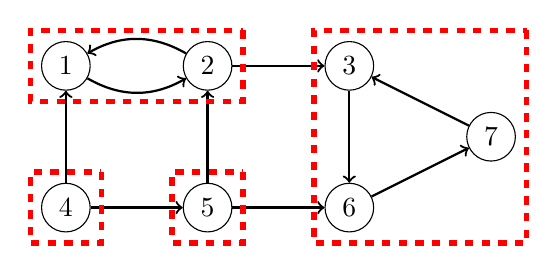
\begin{tikzpicture}[scale=0.9,label distance=-2mm]
\node[draw, circle] (1) at (-1,1) {$7$};
\node[draw, circle] (2) at (-3,2) {$3$};
\node[draw, circle] (4) at (-5,2) {$2$};
\node[draw, circle] (6) at (-7,2) {$1$};
\node[draw, circle] (3) at (-3,0) {$6$};
\node[draw, circle] (5) at (-5,0) {$5$};
\node[draw, circle] (7) at (-7,0) {$4$};

\path[draw,thick,<-] (2) -- (1);
\path[draw,thick,<-] (1) -- (3);
\path[draw,thick,<-] (3) -- (2);
\path[draw,thick,<-] (2) -- (4);
\path[draw,thick,<-] (3) -- (5);
\path[draw,thick,<-] (4) edge [bend left] (6);
\path[draw,thick,<-] (6) edge [bend left] (4);
\path[draw,thick,<-] (4) -- (5);
\path[draw,thick,<-] (5) -- (7);
\path[draw,thick,<-] (6) -- (7);

\draw [red,thick,dashed,line width=2pt] (-0.5,2.5) rectangle (-3.5,-0.5);
\draw [red,thick,dashed,line width=2pt] (-4.5,2.5) rectangle (-7.5,1.5);
\draw [red,thick,dashed,line width=2pt] (-4.5,0.5) rectangle (-5.5,-0.5);
\draw [red,thick,dashed,line width=2pt] (-6.5,0.5) rectangle (-7.5,-0.5);
\end{tikzpicture}
\end{center}
\end{samepage}

A complexidade de tempo do algoritmo é $O(n+m)$,
porque o algoritmo
realiza duas buscas em profundidade.

\section{Problema 2SAT}

\index{problema 2SAT}

A conectividade forte também está relacionada ao
\key{problema 2SAT}\footnote{O algoritmo apresentado aqui foi
introduzido em \cite{asp79}.
Há também outro algoritmo linear conhecido \cite{eve75}
que é baseado em backtracking.}.
Neste problema, recebemos uma fórmula lógica
\[
(a_1 \lor b_1) \land (a_2 \lor b_2) \land \cdots \land (a_m \lor b_m),
\]
onde cada $a_i$ e $b_i$ é uma variável lógica
($x_1,x_2,\ldots,x_n$)
ou uma negação de uma variável lógica
($\lnot x_1, \lnot x_2, \ldots, \lnot x_n$).
Os símbolos ''$\land$'' e ''$\lor$'' denotam
os operadores lógicos ''e'' e ''ou''.
Nossa tarefa é atribuir a cada variável um valor
para que a fórmula seja verdadeira, ou declarar
que isso não é possível.

Por exemplo, a fórmula
\[
L_1 = (x_2 \lor \lnot x_1) \land
      (\lnot x_1 \lor \lnot x_2) \land
      (x_1 \lor x_3) \land
      (\lnot x_2 \lor \lnot x_3) \land
      (x_1 \lor x_4)
\]
é verdadeira quando as variáveis são atribuídas da seguinte forma:

\[
\begin{cases}
x_1 = \textrm{falso} \\
x_2 = \textrm{falso} \\
x_3 = \textrm{verdadeiro} \\
x_4 = \textrm{verdadeiro} \\
\end{cases}
\]

No entanto, a fórmula
\[
L_2 = (x_1 \lor x_2) \land
      (x_1 \lor \lnot x_2) \land
      (\lnot x_1 \lor x_3) \land
      (\lnot x_1 \lor \lnot x_3)
\]
é sempre falsa, independentemente de como
atribuímos os valores.
A razão para isso é que não podemos
escolher um valor para $x_1$
sem criar uma contradição.
Se $x_1$ for falso, ambos $x_2$ e $\lnot x_2$
devem ser verdadeiros, o que é impossível,
e se $x_1$ for verdadeiro, ambos $x_3$ e $\lnot x_3$
devem ser verdadeiros, o que também é impossível.

O problema 2SAT pode ser representado como um grafo
cujos nós correspondem às
variáveis $x_i$ e negações $\lnot x_i$,
e as arestas determinam as conexões
entre as variáveis.
Cada par $(a_i \lor b_i)$ gera duas arestas:
$\lnot a_i \to b_i$ e $\lnot b_i \to a_i$.
Isso significa que se $a_i$ não for verdadeiro,
$b_i$ deve ser verdadeiro, e vice-versa.

O grafo para a fórmula $L_1$ é:
\\
\begin{center}
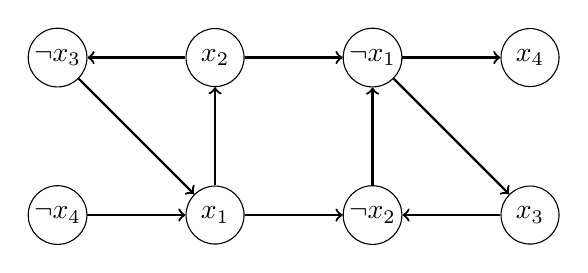
\begin{tikzpicture}[scale=1.0,minimum size=2pt]
\node[draw, circle, inner sep=1.3pt] (1) at (1,2) {$\lnot x_3$};
\node[draw, circle] (2) at (3,2) {$x_2$};
\node[draw, circle, inner sep=1.3pt] (3) at (1,0) {$\lnot x_4$};
\node[draw, circle] (4) at (3,0) {$x_1$};
\node[draw, circle, inner sep=1.3pt] (5) at (5,2) {$\lnot x_1$};
\node[draw, circle] (6) at (7,2) {$x_4$};
\node[draw, circle, inner sep=1.3pt] (7) at (5,0) {$\lnot x_2$};
\node[draw, circle] (8) at (7,0) {$x_3$};
 
\path[draw,thick,->] (1) -- (4);
\path[draw,thick,->] (4) -- (2);
\path[draw,thick,->] (2) -- (1);
\path[draw,thick,->] (3) -- (4);
\path[draw,thick,->] (2) -- (5);
\path[draw,thick,->] (4) -- (7);
\path[draw,thick,->] (5) -- (6);
\path[draw,thick,->] (5) -- (8);
\path[draw,thick,->] (8) -- (7);
\path[draw,thick,->] (7) -- (5);
\end{tikzpicture}
\end{center}
E o grafo para a fórmula $L_2$ é:
\\
\begin{center}
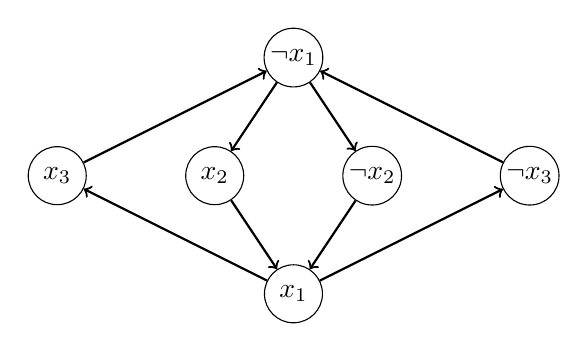
\begin{tikzpicture}[scale=1.0,minimum size=2pt]
\node[draw, circle] (1) at (1,2) {$x_3$};
\node[draw, circle] (2) at (3,2) {$x_2$};
\node[draw, circle, inner sep=1.3pt] (3) at (5,2) {$\lnot x_2$};
\node[draw, circle, inner sep=1.3pt] (4) at (7,2) {$\lnot x_3$};
\node[draw, circle, inner sep=1.3pt] (5) at (4,3.5) {$\lnot x_1$};
\node[draw, circle] (6) at (4,0.5) {$x_1$};

\path[draw,thick,->] (1) -- (5);
\path[draw,thick,->] (4) -- (5);
\path[draw,thick,->] (6) -- (1);
\path[draw,thick,->] (6) -- (4);
\path[draw,thick,->] (5) -- (2);
\path[draw,thick,->] (5) -- (3);
\path[draw,thick,->] (2) -- (6);
\path[draw,thick,->] (3) -- (6);
\end{tikzpicture}
\end{center}

A estrutura do grafo nos diz se
é possível atribuir os valores
das variáveis para
que a fórmula seja verdadeira.
Acontece que isso pode ser feito
exatamente quando não há nós
$x_i$ e $\lnot x_i$ tais que
ambos os nós pertençam ao
mesmo componente fortemente conexo.
Se houver tais nós,
o grafo contém
um caminho de $x_i$ para $\lnot x_i$
e também um caminho de $\lnot x_i$ para $x_i$,
então ambos $x_i$ e $\lnot x_i$ devem ser verdadeiros,
o que não é possível.

No grafo da fórmula $L_1$,
não há nós $x_i$ e $\lnot x_i$
tais que ambos os nós 
pertençam ao mesmo componente fortemente conexo,
então uma solução existe.
No grafo da fórmula $L_2$,
todos os nós pertencem ao mesmo componente fortemente conexo,
então uma solução não existe.

Se uma solução existir, os valores para as variáveis
podem ser encontrados percorrendo os nós do
grafo de componentes em uma ordem de ordenação topológica inversa.
A cada passo, processamos um componente 
que não contém arestas que levam a um
componente não processado.
Se as variáveis no componente
não tiverem sido atribuídas a valores,
seus valores serão determinados
de acordo com os valores no componente,
e se eles já tiverem valores,
eles permanecem inalterados.
O processo continua até que cada variável
tenha sido atribuída a um valor.

O grafo de componentes para a fórmula $L_1$ é o seguinte:
\begin{center}
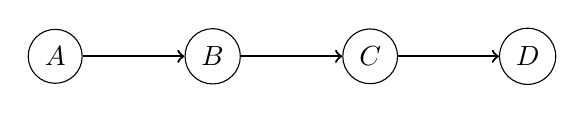
\begin{tikzpicture}[scale=1.0]
\node[draw, circle] (1) at (0,0) {$A$};
\node[draw, circle] (2) at (2,0) {$B$};
\node[draw, circle] (3) at (4,0) {$C$};
\node[draw, circle] (4) at (6,0) {$D$};

\path[draw,thick,->] (1) -- (2);
\path[draw,thick,->] (2) -- (3);
\path[draw,thick,->] (3) -- (4);
\end{tikzpicture}
\end{center}

Os componentes são
$A = \{\lnot x_4\}$,
$B = \{x_1, x_2, \lnot x_3\}$,
$C = \{\lnot x_1, \lnot x_2, x_3\}$ e
$D = \{x_4\}$.
Ao construir a solução,
primeiro processamos o componente $D$
onde $x_4$ se torna verdadeiro.
Depois disso, processamos o componente $C$
onde $x_1$ e $x_2$ se tornam falsos
e $x_3$ se torna verdadeiro.
Todas as variáveis foram atribuídas a valores,
então os componentes restantes $A$ e $B$
não alteram as variáveis.

Observe que este método funciona porque o
grafo tem uma estrutura especial:
se houver caminhos do nó $x_i$ para o nó $x_j$
e do nó $x_j$ para o nó $\lnot x_j$,
então o nó $x_i$ nunca se torna verdadeiro.
A razão para isso é que também há
um caminho do nó $\lnot x_j$ para o nó $\lnot x_i$,
e ambos $x_i$ e $x_j$ se tornam falsos.

\index{problema 3SAT}

Um problema mais difícil é o \key{problema 3SAT},
onde cada parte da fórmula é da forma
$(a_i \lor b_i \lor c_i)$.
Este problema é NP-difícil, então nenhum algoritmo eficiente
para resolver o problema é conhecido.
